\subsection{Execution Plan and Deliverables}
The core program is organized into twelve modules with explicit outputs (Table~\ref{tab:workplan}). The timeline is a proposed eight-week allocation after reagent availability, not a record of work performed. Five additional research modules are specified separately in the next section. Modules advance only after their stated acceptance checks. Figure~\ref{fig:evidence-design} connects the different levels of evidence; arrows indicate the planned order of investigation, not demonstrated causation.

\begin{figure}[htbp]
\centering
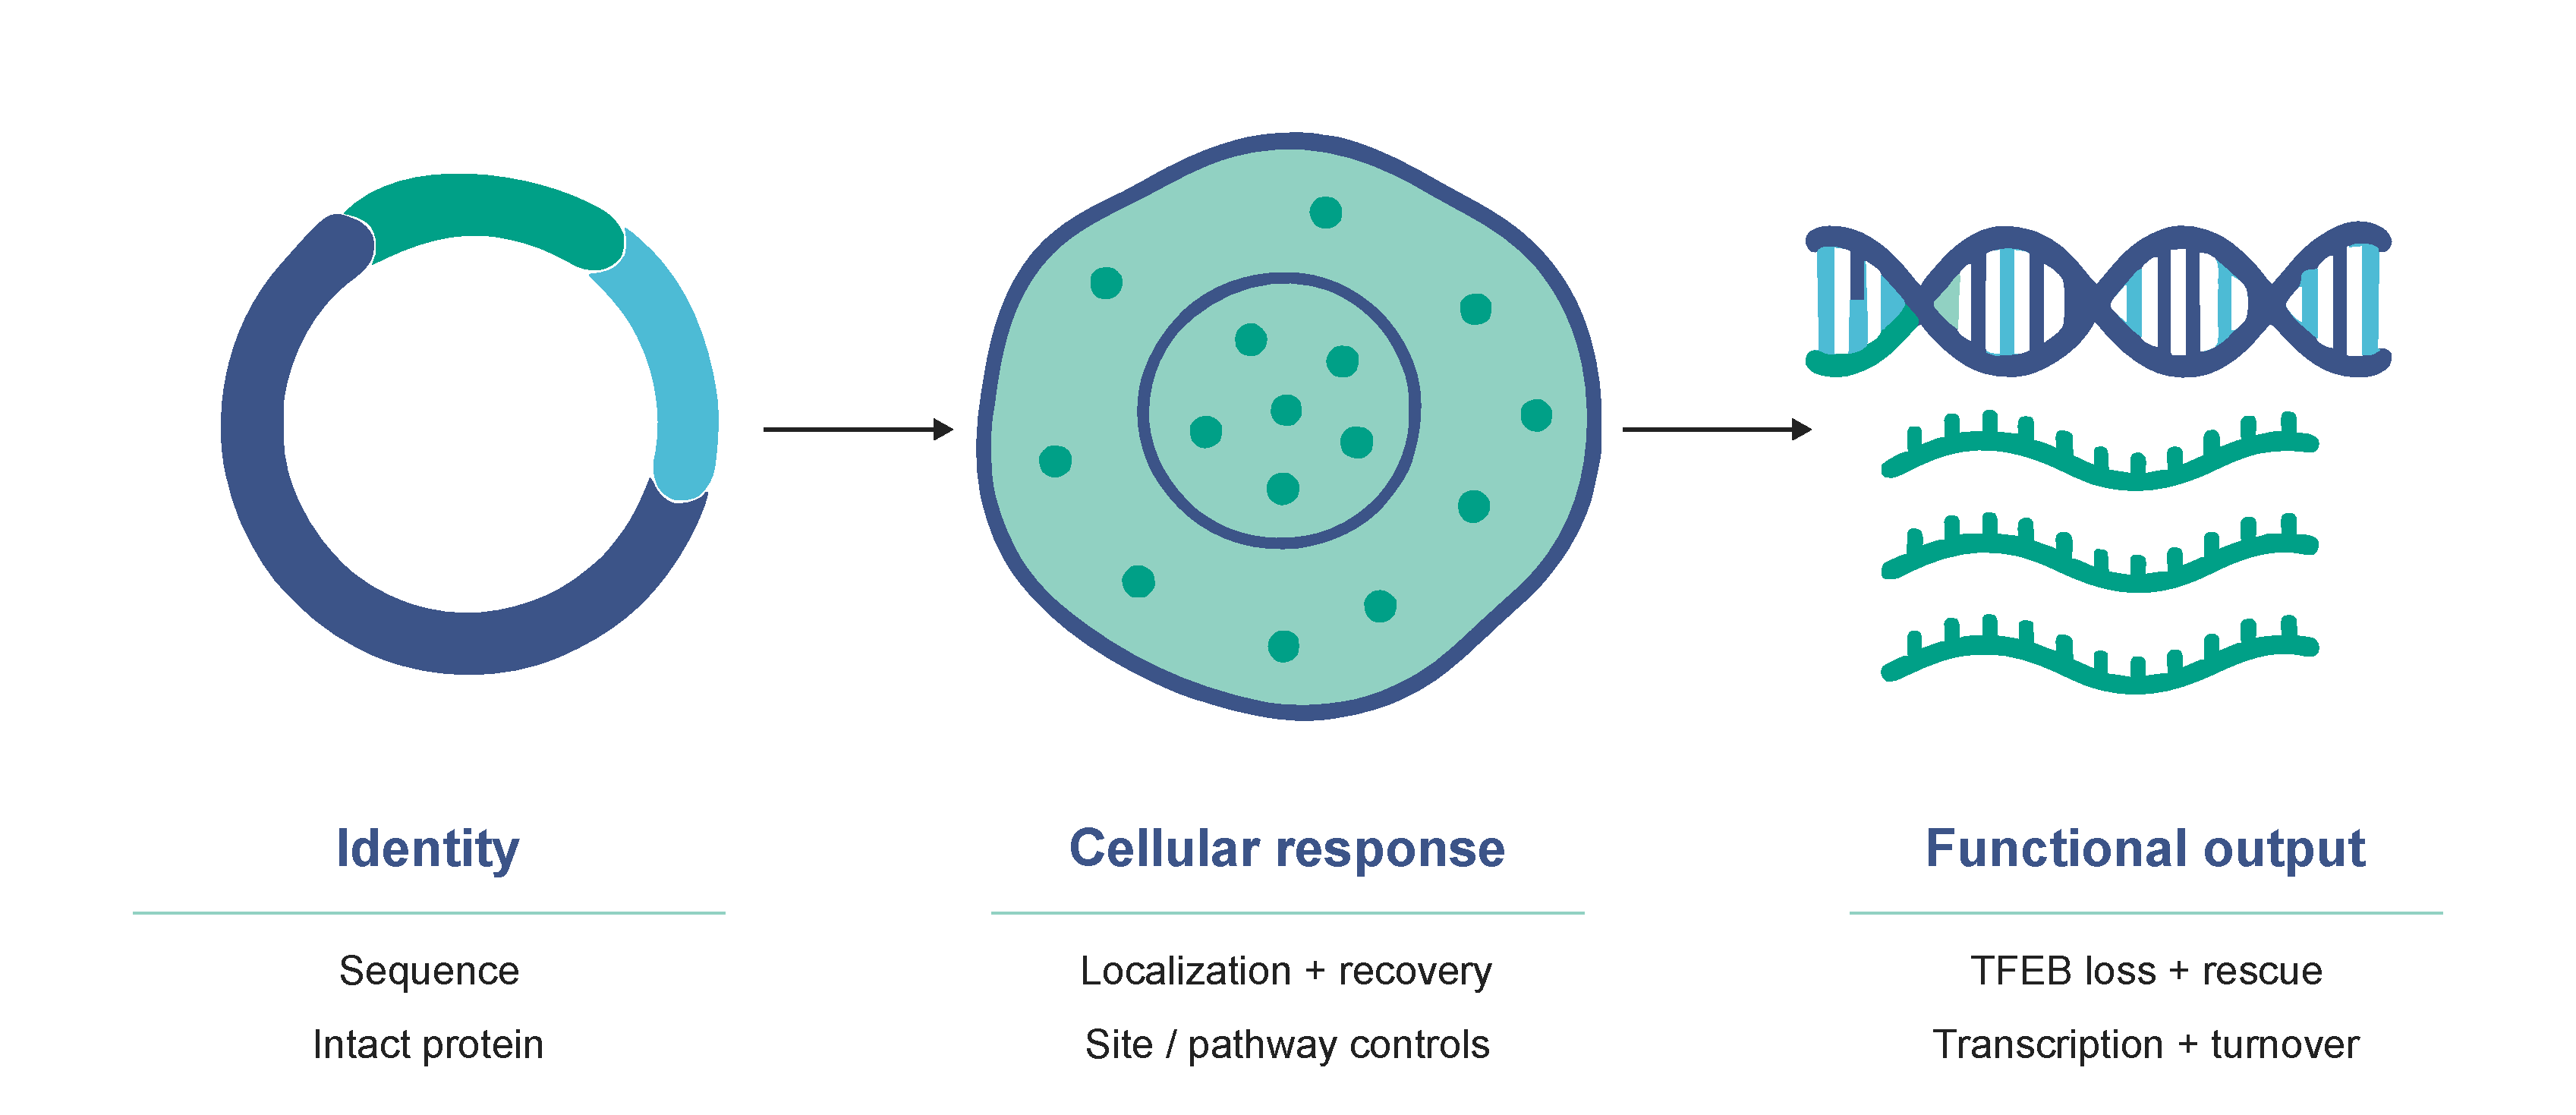
\includegraphics[width=\textwidth]{images/B/evidence-design-imagegen-v3.pdf}
\caption{Evidence structure for the expanded study. Construct identity precedes biological assays; reporter and endogenous localization are checked before site/pathway interpretation. TFEB loss/rescue tests target-gene RNA responses and turnover. The transcription branch requires qualified nascent-RNA evidence for a rate interpretation; turnover requires paired bafilomycin A1 controls. Icons are conceptual drawings, not experimental images. Each stage needs the negative, positive and specificity controls in the methods. Agreement strengthens interpretation; disagreement narrows the conclusion.}
\label{fig:evidence-design}
\end{figure}

\small
\begin{longtable}{L{0.08\textwidth}L{0.10\textwidth}L{0.33\textwidth}L{0.40\textwidth}}
\caption{Proposed workload, acceptance checks and assessable deliverables.}\label{tab:workplan}\\
\toprule ID & Week & Module & Deliverable / acceptance check \\
\midrule\endfirsthead
\toprule ID & Week & Module & Deliverable / acceptance check \\
\midrule\endhead
\bottomrule\endfoot
M01 & 1 & WT and three mutant donor/construct designs & Versioned sequences, five plasmid maps, codon and junction audit. Computational deliverables are provided; material identity still needs verification. \\
M02 & 1--2 & Cloning, selection and clone QC & PCR/digest records, failed-clone log and full bidirectional sequence acceptance; two independent accepted clones per genotype for key checks. \\
M03 & 2--3 & Cell quality and expression pilot & Authentication/mycoplasma record; dose, viability and detector-linearity decisions frozen before confirmation. \\
M04 & 3--4 & WT nutrient and drug response & Matched-media/solvent controls; raw images, masks, per-cell intensities and independent-day N/C summaries. \\
M05 & 4 & Endogenous TFEB and fractionation & Specific endogenous IF; reciprocal fraction-purity checks and volume-corrected partition estimates. \\
M06 & 4--5 & Time course, refeeding and mutants & Four-genotype baseline/treatment and recovery contrasts; matched elapsed-time controls and clone-confirmation record. \\
M07 & 5 & Phosphorylation and pathway readouts & Uncropped p-TFEB, p-S6K and total-protein blots; S211A and phosphatase specificity checks. \\
M08 & 5--6 & RPTOR versus RICTOR RNAi & Two individual siRNAs per target, knockdown and pathway-engagement evidence; qualified complex-attribution conclusion. \\
M09 & 6 & 14-3-3 association & GFP capture with input, EGFP-only and beads-only controls; association normalized to recovered bait. \\
M10 & 6--7 & TFEB loss and WT rescue & Two independent 3$'$-UTR siRNAs; endogenous depletion, verified rescue expression and control-siRNA + WT arm. \\
M11 & 7--8 & Transcription and turnover & Validated qPCR assays and paired inhibitor/no-inhibitor LC3-II contrasts; p62 transcript/protein and viability. \\
M12 & 8 & Integration and reproducibility & Blinded analysis record, exclusions, effect estimates with intervals, source data, figure legends and alternative-interpretation table. \\
\end{longtable}
\normalsize

For a concrete workload example, the four fusion genotypes crossed with three matched 60-min conditions (fed vehicle, amino-acid deprivation with vehicle, and fed Torin1) yield 12 conditions. Four independent days with two technical wells per condition require 96 assay wells and at least 2,880 eligible cells at 30 cells per well. These are planning quantities, not observations; they exclude parental/mock/EGFP-only controls, pilot wells, recovery time points, protein/RNA plates and repeat attempts. A separate plate map must enumerate those additions before execution. Independent-day replication must not be replaced by more cells from one day. The larger program is divided into modules to keep each comparison interpretable and scheduling feasible.

The report currently supplies design figures and computational sequence checks. Experimental image, blot, qPCR and turnover panels are planned outputs and will only be populated with acquired data. Before running M08--M11, finalize exact siRNA targets, qPCR oligos and reagent identities and verify their performance; these are open execution items rather than completed designs.
\FloatBarrier
